%%%%%%%%%%%%%%%%%%%%%%%%%%%%%%%%%%%%%%%%%%%%%%%%%%%%%%%%%%%%%%%%%%%%%%%%%%%%%%%%
%2345678901234567890123456789012345678901234567890123456789012345678901234567890
%        1         2         3         4         5         6         7         8

%\documentclass[letterpaper, 10 pt, conference]{ieeeconf}  % Comment this line out
                                                          % if you need a4paper
\documentclass[a4paper, 10pt, conference]{ieeeconf}      % Use this line for a4
                                                          % paper

\IEEEoverridecommandlockouts                              % This command is only
                                                          % needed if you want to
                                                          % use the \thanks command
\overrideIEEEmargins
% See the \addtolength command later in the file to balance the column lengths
% on the last page of the document



% The following packages can be found on http:\\www.ctan.org
\usepackage{graphics} % for pdf, bitmapped graphics files
%\usepackage{epsfig} % for postscript graphics files
%\usepackage{mathptmx} % assumes new font selection scheme installed
%\usepackage{times} % assumes new font selection scheme installed
%\usepackage{amsmath} % assumes amsmath package installed
%\usepackage{amssymb}  % assumes amsmath package installed

\title{\LARGE \bf
Practical Tutorial for SDR using GNU Radio
}

%\author{ \parbox{3 in}{\centering Huibert Kwakernaak*
%         \thanks{*Use the $\backslash$thanks command to put information here}\\
%         Faculty of Electrical Engineering, Mathematics and Computer Science\\
%         University of Twente\\
%         7500 AE Enschede, The Netherlands\\
%         {\tt\small h.kwakernaak@autsubmit.com}}
%         \hspace*{ 0.5 in}
%         \parbox{3 in}{ \centering Pradeep Misra**
%         \thanks{**The footnote marks may be inserted manually}\\
%        Department of Electrical Engineering \\
%         Wright State University\\
%         Dayton, OH 45435, USA\\
%         {\tt\small pmisra@cs.wright.edu}}
%}


\author{André Silva$^{1}$
\thanks{*This work was supported by Instituto de Telecomunicações}% <-this % stops a space
\thanks{$^{1}$André Silva is with Faculty of Sciences and Technology,
        University of Coimbra, Portugal}
}

\begin{document}

\maketitle
\thispagestyle{empty}
\pagestyle{empty}


%%%%%%%%%%%%%%%%%%%%%%%%%%%%%%%%%%%%%%%%%%%%%%%%%%%%%%%%%%%%%%%%%%%%%%%%%%%%%%%%
\begin{abstract}

This electronic document is a ÒliveÓ template. The various components of your paper [title, text, heads, etc.] are already defined on the style sheet, as illustrated by the portions given in this document.

\end{abstract}


%%%%%%%%%%%%%%%%%%%%%%%%%%%%%%%%%%%%%%%%%%%%%%%%%%%%%%%%%%%%%%%%%%%%%%%%%%%%%%%%
\section{INTRODUCTION}

SOMETHING

\section{GETTING STARTED}
We need a Linux base for getting started, this installing guide was meant to Ubuntu 18.04 or the Ubuntu 19.04.
\subsection{Installing VOLK}
First of all we will install VOLK (Vector-Optimized Library of Kernels) because we will not use the internal VOLK of GNU Radio but an external one. VOLK it's a free library that contains kernels for mathematical operations, this means that for an operation is created a proto-kernel and added to VOLK for the architecture that we wish, hence faster operations. To install this follow the next commands:
\begin{itemize}
    \item git clone https://github.com/gnuradio/volk
    \item cd volk \&\& mkdir build \&\& cd build
    \item cmake ..\/
    \item make \&\& make test \&\& sudo make install \&\& sudo ldconfig
\end{itemize}

To complete this, we need to create a profile for our architecture, for this go to "/usr/bin/" folder and run "volk\_profile". Note that the configuration file is written in the next path: "\$HOME/.volk/volk\_config".

\subsection{Installing GNU Radio}
Now moving for GNU Radio, the first thing to do is install all the dependencies needed, with the next command:


"sudo apt install cmake git g++ libboost-all-dev python-dev python-mako python-numpy python-wxgtk3.0 python-sphinx python-cheetah swig libzmq3-dev libfftw3-dev libgsl-dev libcppunit-dev doxygen libcomedi-dev libqt4-opengl-dev python-qt4 libqwt-dev libsdl1.2-dev libusb-1.0-0-dev python-gtk2 python-lxml pkg-config python-sip-dev"


After dependencies installed we will install GNU Radio via git. It is available the Version 3.8 however still has a lot of stability problems and bugs so we keep with the last commit of 3.7 version:
\begin{itemize}
    \item git clone https://github.com/gnuradio/gnuradio.git
    \item cd gnuradio \&\& git checkout maint-3.7
    \item mkdir build \&\& cd build
    \item cmake -DENABLE\_INTERNAL\_VOLK=OFF ..\/
    \item make \&\& make test \&\& sudo make install \&\& sudo ldconfig
\end{itemize}

You can now use the GNU Radio, to see where was installed where it is a usefull command: "which gnuradio-companion".

\subsection{Installing UHD Driver}
To use the USRP's we need to install the UHD Driver, and for that we install three packages:
libuhd-dev, libuhd3.14.1 and uhd-host.
This packages can be downloaded here:
https://launchpad.net/~ettusresearch/+archive/ubuntu/uhd/+packages

Finally to download the image of your USRP just run: 
"./uhd\_images\_downloader.py" inside the folder "/usr/lib/uhd/utils/".

If everything works you can run the next command to see the devices connected:
"uhd\_find\_devices", and this one to see information about that devices: "uhd\_usrp\_probe".


\subsection{Problems and Solutions}
After installing GNU Radio when you open it if shows some warnings about "Camberra" just install it with "sudo apt install libcanberra-gtk-module libcanberra-gtk3-module"

\section{GUIDED TUTORIAL - MODULATION}

BALBLABLA

\subsection{Modulation - Tutorial\_1.grc}
    In order to transmit data between SDR's it's necessary modulate the signal, so the modulation is the act of varying properties of a waveform, this wave is called carrier and keeps the information transmitted, so the the goal here is pick the data and modulate it so it can be transmitted.
    
    First we need to understand the working of some blocks and hence the GNU Radio itself. 
    
    %-----------
    
    We can convert bytes in complex numbers using the "Chunks to Symbols" block, this block has a parameter called "Symbol Table" where we define the mapping between a byte (a chunk, this is our symbol) and a constellation point (point in the constellation to the symbol). But before we need to do two things:
        First we need to unpack the byte, this means split the 8 bits/byte in X significant bits/byte being X the number of bits necessary to the symbol of the constellation type, this is, if we want modulate in BPSK X is 1, QPSK X is 2, 8PSK X is 4.
        This is possible using the "Repack Bits" block, this block has 3 important parameters, the "Bits per Input Byte" where we define how many bits we pick in an incoming byte, the "Bits per Output Byte" where we define how many significant bits will have the output byte (the remaining bits will be 0's), and finally the parameter "Endianness" to determinate if we want write in MSB or LSB (always read in LSB). 
        For example if we input the byte = "01000010":
        With 8:2 in MSB we got:"000000\textbf{01}", "000000\textbf{00}", "000000\textbf{00}", "000000\textbf{10}".
        With 8:2 in LSB we got:"000000\textbf{10}", "000000\textbf{00}", "000000\textbf{00}", "000000\textbf{01}".
    Note that this block leads to an interpolation of "Bits per Output Byte/Bits per Input Byte, in this case 8/2=4, this is, for every 1 bytes outputs 4 bytes". 
        
        Second we need to map the resulting bits in the symbols that we really want, using the "Map" block that basically does: output[i] = map[input[i]].
    
    Lets suppose we want modulate using QPSK: 
        First we create an "Constellation Object" where we insert the mapping of the symbols relative to the constellation points. 
        We need to pick the 8 bits/byte and slicing in 2 significant bits per byte, so we use the "repack bits" with 8 "Bits per Input Byte" and 2 "Bits per output Byte" with MSB endianness. Currently we have a byte with the first 6 bits with 0's and the next 2 bits with 2 bits of data, however it's not our symbol wet).
        Then we map this significant 2 bits in the symbol we want taking into account that we will map this symbols in constellation points next (using the "Constellation object" block). In this case the 2 significant bits coincide with the symbol, but it depends of what you want to do.
        Resulting in mapping into the constellation points in the \ref{fig:mapping_qpsk}
        \begin{figure}
            \centering
            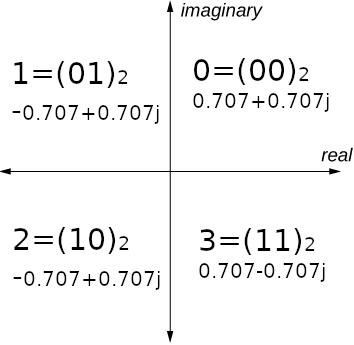
\includegraphics{mapping_qpsk.jpg}
            \caption{QPSK: Mapping Symbols to Constellation Points}
            \label{fig:mapping_qpsk}
        \end{figure}
        
        The last block is "Throttle", to understand this block we need understand how GR works. When we do data streaming, we are implicitly using a buffers to hold the data between blocks, this buffers are in finite size so before the block do anything, it checks the amount of available space in input and output buffers, if there is none available space in that buffers the block don't do anything. This is called "Back-pressure" because we pressure back the data that is incoming, slowing things down. This is how GR controls the data flow, giving data to the block when it's necessary and holding it when block is busy working. We have source/sink blocks that produces/consumes data at a given fixed sample rate like Audio and USRP blocks, these blocks are called "clock" blocks, so typically a FG has only or one source or one sink, and not both because that leads to an problem called as "2 clock problem" where there is 2 blocks with different sample rates leading a asynchronous clock sources causing "underruns"/"overflows" depending on the production/consumption rates are differentiating. As our FG doesn't has any of this "clock" blocks then we need to add the "Throttle" block to act as a clock, without it the FG will run as fast as the CPU can process resulting in non-responsive program and other problems. This means that while we are in simulating mode we need this block to control the flow however when we start using the "USRP" blocks we can take out this block.
        
        To finalize the TX side we send the data to an virtual sink, that redirects the data to the virtual source with the same id, the only purpose of this block it's make the FG more clear, elegant and readable.
        
        Now we move to the RX part of the FG where we use the "Constellation Decoder" to invert what we have done, this is, map the complex points to symbols (using the parameters of the "he "Constellation Object" block), and then we use "Map" block again to map symbols into bits of real data. And then pick the 2 significant bits and pack in a byte exactly the inverse as before.
        
        
\subsection{Modulation - Tutorial\_2.grc}
    What we have done is not enough because in real world we cant use all the bandwidth, so we need no narrow it, however if the channels are too narrow the symbols will be too wide and the tail of the last symbol will interfere with the present one inducing ISI (Inter-Symbol Interference). A pulse shaping filter we can use to work around is the RRC (Root Raised Cosine) filter because it's a feasible solution and it's implemented in GR.      
    
    %--------RRC filter
   If we did not put a shaping filter on the signal, the waves will produce have a lot of energy in adjacent channels. This filter uses taps to apply against our signal shaping it. This taps are calculated based in how many number of filters we want and how many samples we want per symbol. Theoretically has an infinite number of taps hence we can infinite attenuate the stop band, so really we can define the limit according with processing power we have. Remember that we have introduced ISI here that we will have to treat in RX side, as we will see.
   

    %Roll off
    
    Another thing to keep in mind is the roll-off factor, this is the measure of the excess bandwidth of the filter (bandwidth that is occupied beyond Nyquist bandwidth). This parameter is basically the inclination of the wave when rising and falling, when we set more roll-off, let's say 1, then will be easier for the receiver to decode however we will narrow less the bandwidth and that is not our objective, on the other hand, smaller roll-off will result in narrower bandwidth, however the inclination increases so attenuation in stop band is reduced.
    I provide an FG that made called "roll\_off.grc" inside of "extra" folder where you can analyse the plot of 5 different roll-off factors. In this tutorial we will use the 0.22 value to this parameter.
    %-filter delay.
    %--Decreasing the number of samples (filter delay) reduces the stop band attenuation.
    
    %---SPS
    Another thing to do in modulation is the interpolation, so basically we can set a number of SPS ( samples per symbol) that we can however, logically, more samples per symbol leads to less probability of errors hence induced more overhead to our transmission. What this does is construct new points in the wave between the existing ones hence we are reconstructing the signal we will be a lot more precise. To find this parameter we have 2 criteria:  First leaving this values small as possible taking into account that is mandatory be 2 or higher. Second we can use this value to help us match the desired bit rate taking into account the sample rate of the hardware we are using, (currently none but we will use USRP's). We will use 4 for this parameter.
    
    %--------RX SIDE - chega??
    Note that at this point we have ISI in our signal, so first I have to get rid of this by using another RRC filter. When we combine 2 RRC filter together we get a RRC filter with Nyquist filter form. Knowing this property we can use another RRC filter resulting in a raised cosine pulse shaped filter with less ISI. If you observe the constellation plot "RX Treated Constellation" there is a little noisy as a result of the ISI after the 32 filters however much less noisy than "RX Constellation". 
    %--SPS 4-1
    Now that we have applied a RRC filter to our RX signal, in the same way that we have re-sampling by 4 we need to decimate to converting 4 samples per symbol into only 1 sample per symbol.

\subsection{Modulation - Tutorial\_3.grc}
    Now we are ready no get closer to reality, for that let's implement a "Channel Model" block where simulates different properties of a channel that we will need to take care:
    
\begin{itemize}
\item Noise - We can add Additive White Gaussian Noise (AWGN) in parameter "Noise Voltage" where we set a level as a voltage;
\item Frequency Offset - The "Frequency\_offset" parameter where 0 is no offset and 0.25 would be a digital modem (1/4 of the symbol rate);
\item Timing Offset - The "Epsilon" parameter allows emulating different sample clocks between the transmitter e the receiver and 1.0 is no offset added.
\item Multipath - We can emulate multipath delay by adding taps of a FIR (Finite Impulse Response) filter in the "Taps" parameter.
\end{itemize}
    
    
    The FG we have is already taken care of noise and timing offset using the "Polyphase Clock Sync" block. If you play with the tweaks "Time Offset" and "Noise Amp" you can see in the plot of "Rx Treated constellation" a nice and clear constellation, however if you tweak the "Freq Offset" you can see that the constellation become a circle, that's because we are not treating that, it will be what we will do next tutorial.
    
\subsection{Modulation - Tutorial\_4.grc}
    %O que é multipath - tratar MULTIPATH
    Multipath is having different paths to our receptor, for example when using wireless the signal  reflects on objects of the environment, for example walls and go to receptor a little after the direct path, so the receptor receives the same signal various times with timing differences. 
    I added some taps to simulate a multipah property, if you disable "Costas Loop" and the "CMA Equalizer" and set "Output SPS" to 1 in the "Polyphase Clock Sync" block you can see the effect of these taps because the constellation points are no longer clean and really converged: \ref{fig:multipath_effect}

    \begin{figure}
        \centering
        \includegraphics{multipath_effect}
        \caption{Effects Multipath on Constellation Plot}
        \label{fig:multipath_effect}
    \end{figure}
    
    This, obviously affects our transmission so to take we will need an equalizer, called "CMA equalizer". Here we define the number of taps, more taps means more overhead to the algorithm so we want keep this number small but enough for correcting our channel (based on educated guess, I set 15 because works with other implementations and is enough for now). The "Gain" I set 0.01 and the "Samples per Symbol" of the input signal is set to "2", hence, the "Output SPS" of "Polyphase Clock Sync" block is also set to "2". If you take a look now for the constellation plot you will see a constellation a lot more converged and clean: \ref{fig:multipath_corrected}
    \ref{fig:multipath_effect}

    \begin{figure}
        \centering
        \includegraphics{multipath_corrected}
        \caption{Multipath corrected on Constellation Plot}
        \label{fig:multipath_corrected}
    \end{figure}
    
    %TRATAR Frequency offset 
    Note that the constellation is rotating, thats because of the little frquency offset iposed by "CMA Equalizer" block. If you tweak the Freq Time you will see an circle insted a constellation, that is what we need to take care, the last property is the frequency offset.
    
        %----------------------___FIQUEI AQUI---------------EXPLICAR O COSTASS LOOP
    
    



\subsection{Packet communications - Tutorial\_5.grc}
    Now we have successfully modulated and transmitted our signal, but if you take a look in the output file, will only be junk. This is happening because it's not writing the bits in the supposed byte. Explaining better, if I send the byte "01010101" and for some motive receives 4 bits in 0's and then the right bye, this results in "0000\textbf{0101}" and "\textbf{0101}XXXX", then all the bits forward are not aligned. This is the problem that is happening here, so we need a manner to always receive the bytes aligned. The solution for this is packetize our data and send the packet.
    
    %CAC
    The first thing we need to know is how the "Correlate Access Code - Tag Stream" block works. It expect unpacked data, this means that the input only has 1 significant bit per byte. Then examining the input finds the sequence called "Access Code" of 64 bits taking into account that can be X bits different where X is the "Threshold" parameter. After find this sequence the next 32 bits is the length of the payload (that will be outputted) repeated twice. Resulting in a header with 64 bits of access code, 16 bits of payload length and another 16 bits of payload length. The length of the payload is in bytes. Now that we have the composition of the header of the packet we need to create it.
    
    %Inicio
    Assuming that we want transmit packets with 112 bytes of payload size, hence 896 bits, then we need to create the header with that information. 
    %-Create header
    To create the header we will use the "Vector Source" block with the "Repeat" parameter set to "Yes", and the vector will be 64 bits of the access code (I will use the default that can be accessed here "digital.packet\_utils.default\_access\_code"), followed by "00000000 01110000" = 112 and then "00000000 01110000" = 112. With header ready we need to split the input in 1 bit/byte using "Repack Bits" block mentioned before, then concatenate the 96 bits of the header with 896 bits of the payload using "Stream Mux" block, and finally repack again to 2 bits/byte resulting in the packet ready to modulate and transmit.
    
    %RX
    At the RX side we just need to repack to 1 bit/byte to use the "Correlate Access Code - Tag Stream" block and extract the payload of the packet and repack to 8 bits/byte. Now if you take a look at the output file you see that the bits are alygned correctly in the byte nedded.
    
\subsection{Packet communications - Tutorial\_4.grc}
    It seems eve


\subsection{Units}

\begin{itemize}

\item Use either SI (MKS) or CGS as primary units. (SI units are encouraged.) English units may be used as secondary units (in parentheses). An exception would be the use of English units as identifiers in trade, such as Ò3.5-inch disk driveÓ.
\item Avoid combining SI and CGS units, such as current in amperes and magnetic field in oersteds. This often leads to confusion because equations do not balance dimensionally. If you must use mixed units, clearly state the units for each quantity that you use in an equation.
\item Do not mix complete spellings and abbreviations of units: ÒWb/m2Ó or Òwebers per square meterÓ, not Òwebers/m2Ó.  Spell out units when they appear in text: Ò. . . a few henriesÓ, not Ò. . . a few HÓ.
\item Use a zero before decimal points: Ò0.25Ó, not Ò.25Ó. Use Òcm3Ó, not ÒccÓ. (bullet list)

\end{itemize}


\subsection{Equations}

The equations are an exception to the prescribed specifications of this template. You will need to determine whether or not your equation should be typed using either the Times New Roman or the Symbol font (please no other font). To create multileveled equations, it may be necessary to treat the equation as a graphic and insert it into the text after your paper is styled. Number equations consecutively. Equation numbers, within parentheses, are to position flush right, as in (1), using a right tab stop. To make your equations more compact, you may use the solidus ( / ), the exp function, or appropriate exponents. Italicize Roman symbols for quantities and variables, but not Greek symbols. Use a long dash rather than a hyphen for a minus sign. Punctuate equations with commas or periods when they are part of a sentence, as in

$$
\alpha + \beta = \chi \eqno{(1)}
$$

Note that the equation is centered using a center tab stop. Be sure that the symbols in your equation have been defined before or immediately following the equation. Use Ò(1)Ó, not ÒEq. (1)Ó or Òequation (1)Ó, except at the beginning of a sentence: ÒEquation (1) is . . .Ó

\subsection{Some Common Mistakes}
\begin{itemize}


\item The word ÒdataÓ is plural, not singular.
\item The subscript for the permeability of vacuum ?0, and other common scientific constants, is zero with subscript formatting, not a lowercase letter ÒoÓ.
\item In American English, commas, semi-/colons, periods, question and exclamation marks are located within quotation marks only when a complete thought or name is cited, such as a title or full quotation. When quotation marks are used, instead of a bold or italic typeface, to highlight a word or phrase, punctuation should appear outside of the quotation marks. A parenthetical phrase or statement at the end of a sentence is punctuated outside of the closing parenthesis (like this). (A parenthetical sentence is punctuated within the parentheses.)
\item A graph within a graph is an ÒinsetÓ, not an ÒinsertÓ. The word alternatively is preferred to the word ÒalternatelyÓ (unless you really mean something that alternates).
\item Do not use the word ÒessentiallyÓ to mean ÒapproximatelyÓ or ÒeffectivelyÓ.
\item In your paper title, if the words Òthat usesÓ can accurately replace the word ÒusingÓ, capitalize the ÒuÓ; if not, keep using lower-cased.
\item Be aware of the different meanings of the homophones ÒaffectÓ and ÒeffectÓ, ÒcomplementÓ and ÒcomplimentÓ, ÒdiscreetÓ and ÒdiscreteÓ, ÒprincipalÓ and ÒprincipleÓ.
\item Do not confuse ÒimplyÓ and ÒinferÓ.
\item The prefix ÒnonÓ is not a word; it should be joined to the word it modifies, usually without a hyphen.
\item There is no period after the ÒetÓ in the Latin abbreviation Òet al.Ó.
\item The abbreviation Òi.e.Ó means Òthat isÓ, and the abbreviation Òe.g.Ó means Òfor exampleÓ.

\end{itemize}


\section{USING THE TEMPLATE}

Use this sample document as your LaTeX source file to create your document. Save this file as {\bf root.tex}. You have to make sure to use the cls file that came with this distribution. If you use a different style file, you cannot expect to get required margins. Note also that when you are creating your out PDF file, the source file is only part of the equation. {\it Your \TeX\ $\rightarrow$ PDF filter determines the output file size. Even if you make all the specifications to output a letter file in the source - if you filter is set to produce A4, you will only get A4 output. }

It is impossible to account for all possible situation, one would encounter using \TeX. If you are using multiple \TeX\ files you must make sure that the ``MAIN`` source file is called root.tex - this is particularly important if your conference is using PaperPlaza's built in \TeX\ to PDF conversion tool.

\subsection{Headings, etc}

Text heads organize the topics on a relational, hierarchical basis. For example, the paper title is the primary text head because all subsequent material relates and elaborates on this one topic. If there are two or more sub-topics, the next level head (uppercase Roman numerals) should be used and, conversely, if there are not at least two sub-topics, then no subheads should be introduced. Styles named ÒHeading 1Ó, ÒHeading 2Ó, ÒHeading 3Ó, and ÒHeading 4Ó are prescribed.

\subsection{Figures and Tables}

Positioning Figures and Tables: Place figures and tables at the top and bottom of columns. Avoid placing them in the middle of columns. Large figures and tables may span across both columns. Figure captions should be below the figures; table heads should appear above the tables. Insert figures and tables after they are cited in the text. Use the abbreviation ÒFig. 1Ó, even at the beginning of a sentence.

\begin{table}[h]
\caption{An Example of a Table}
\label{table_example}
\begin{center}
\begin{tabular}{|c||c|}
\hline
One & Two\\
\hline
Three & Four\\
\hline
\end{tabular}
\end{center}
\end{table}


   \begin{figure}[thpb]
      \centering
      \framebox{\parbox{3in}{We suggest that you use a text box to insert a graphic (which is ideally a 300 dpi TIFF or EPS file, with all fonts embedded) because, in an document, this method is somewhat more stable than directly inserting a picture.
}}
      %\includegraphics[scale=1.0]{figurefile}
      \caption{Inductance of oscillation winding on amorphous
       magnetic core versus DC bias magnetic field}
      \label{figurelabel}
   \end{figure}
   

Figure Labels: Use 8 point Times New Roman for Figure labels. Use words rather than symbols or abbreviations when writing Figure axis labels to avoid confusing the reader. As an example, write the quantity ÒMagnetizationÓ, or ÒMagnetization, MÓ, not just ÒMÓ. If including units in the label, present them within parentheses. Do not label axes only with units. In the example, write ÒMagnetization (A/m)Ó or ÒMagnetization {A[m(1)]}Ó, not just ÒA/mÓ. Do not label axes with a ratio of quantities and units. For example, write ÒTemperature (K)Ó, not ÒTemperature/K.Ó

\section{CONCLUSIONS}

A conclusion section is not required. Although a conclusion may review the main points of the paper, do not replicate the abstract as the conclusion. A conclusion might elaborate on the importance of the work or suggest applications and extensions. 

\addtolength{\textheight}{-12cm}   % This command serves to balance the column lengths
                                  % on the last page of the document manually. It shortens
                                  % the textheight of the last page by a suitable amount.
                                  % This command does not take effect until the next page
                                  % so it should come on the page before the last. Make
                                  % sure that you do not shorten the textheight too much.

%%%%%%%%%%%%%%%%%%%%%%%%%%%%%%%%%%%%%%%%%%%%%%%%%%%%%%%%%%%%%%%%%%%%%%%%%%%%%%%%



%%%%%%%%%%%%%%%%%%%%%%%%%%%%%%%%%%%%%%%%%%%%%%%%%%%%%%%%%%%%%%%%%%%%%%%%%%%%%%%%



%%%%%%%%%%%%%%%%%%%%%%%%%%%%%%%%%%%%%%%%%%%%%%%%%%%%%%%%%%%%%%%%%%%%%%%%%%%%%%%%
\section*{APPENDIX}

Appendixes should appear before the acknowledgment.

\section*{ACKNOWLEDGMENT}

The preferred spelling of the word ÒacknowledgmentÓ in America is without an ÒeÓ after the ÒgÓ. Avoid the stilted expression, ÒOne of us (R. B. G.) thanks . . .Ó  Instead, try ÒR. B. G. thanksÓ. Put sponsor acknowledgments in the unnumbered footnote on the first page.



%%%%%%%%%%%%%%%%%%%%%%%%%%%%%%%%%%%%%%%%%%%%%%%%%%%%%%%%%%%%%%%%%%%%%%%%%%%%%%%%

References are important to the reader; therefore, each citation must be complete and correct. If at all possible, references should be commonly available publications.



\begin{thebibliography}{99}

\bibitem{c1} G. O. Young, ÒSynthetic structure of industrial plastics (Book style with paper title and editor),Ó    in Plastics, 2nd ed. vol. 3, J. Peters, Ed.  New York: McGraw-Hill, 1964, pp. 15Ð64.
\bibitem{c2} W.-K. Chen, Linear Networks and Systems (Book style).  Belmont, CA: Wadsworth, 1993, pp. 123Ð135.
\bibitem{c3} H. Poor, An Introduction to Signal Detection and Estimation.   New York: Springer-Verlag, 1985, ch. 4.
\bibitem{c4} B. Smith, ÒAn approach to graphs of linear forms (Unpublished work style),Ó unpublished.
\bibitem{c5} E. H. Miller, ÒA note on reflector arrays (Periodical styleÑAccepted for publication),Ó IEEE Trans. Antennas Propagat., to be publised.
\bibitem{c6} J. Wang, ÒFundamentals of erbium-doped fiber amplifiers arrays (Periodical styleÑSubmitted for publication),Ó IEEE J. Quantum Electron., submitted for publication.
\bibitem{c7} C. J. Kaufman, Rocky Mountain Research Lab., Boulder, CO, private communication, May 1995.
\bibitem{c8} Y. Yorozu, M. Hirano, K. Oka, and Y. Tagawa, ÒElectron spectroscopy studies on magneto-optical media and plastic substrate interfaces(Translation Journals style),Ó IEEE Transl. J. Magn.Jpn., vol. 2, Aug. 1987, pp. 740Ð741 [Dig. 9th Annu. Conf. Magnetics Japan, 1982, p. 301].
\bibitem{c9} M. Young, The Techincal Writers Handbook.  Mill Valley, CA: University Science, 1989.
\bibitem{c10} J. U. Duncombe, ÒInfrared navigationÑPart I: An assessment of feasibility (Periodical style),Ó IEEE Trans. Electron Devices, vol. ED-11, pp. 34Ð39, Jan. 1959.
\bibitem{c11} S. Chen, B. Mulgrew, and P. M. Grant, ÒA clustering technique for digital communications channel equalization using radial basis function networks,Ó IEEE Trans. Neural Networks, vol. 4, pp. 570Ð578, July 1993.
\bibitem{c12} R. W. Lucky, ÒAutomatic equalization for digital communication,Ó Bell Syst. Tech. J., vol. 44, no. 4, pp. 547Ð588, Apr. 1965.
\bibitem{c13} S. P. Bingulac, ÒOn the compatibility of adaptive controllers (Published Conference Proceedings style),Ó in Proc. 4th Annu. Allerton Conf. Circuits and Systems Theory, New York, 1994, pp. 8Ð16.
\bibitem{c14} G. R. Faulhaber, ÒDesign of service systems with priority reservation,Ó in Conf. Rec. 1995 IEEE Int. Conf. Communications, pp. 3Ð8.
\bibitem{c15} W. D. Doyle, ÒMagnetization reversal in films with biaxial anisotropy,Ó in 1987 Proc. INTERMAG Conf., pp. 2.2-1Ð2.2-6.
\bibitem{c16} G. W. Juette and L. E. Zeffanella, ÒRadio noise currents n short sections on bundle conductors (Presented Conference Paper style),Ó presented at the IEEE Summer power Meeting, Dallas, TX, June 22Ð27, 1990, Paper 90 SM 690-0 PWRS.
\bibitem{c17} J. G. Kreifeldt, ÒAn analysis of surface-detected EMG as an amplitude-modulated noise,Ó presented at the 1989 Int. Conf. Medicine and Biological Engineering, Chicago, IL.
\bibitem{c18} J. Williams, ÒNarrow-band analyzer (Thesis or Dissertation style),Ó Ph.D. dissertation, Dept. Elect. Eng., Harvard Univ., Cambridge, MA, 1993. 
\bibitem{c19} N. Kawasaki, ÒParametric study of thermal and chemical nonequilibrium nozzle flow,Ó M.S. thesis, Dept. Electron. Eng., Osaka Univ., Osaka, Japan, 1993.
\bibitem{c20} J. P. Wilkinson, ÒNonlinear resonant circuit devices (Patent style),Ó U.S. Patent 3 624 12, July 16, 1990. 






\end{thebibliography}




\end{document}
